\documentclass{standalone}
\usepackage{tikz}
\usetikzlibrary{patterns, positioning}


\begin{document}
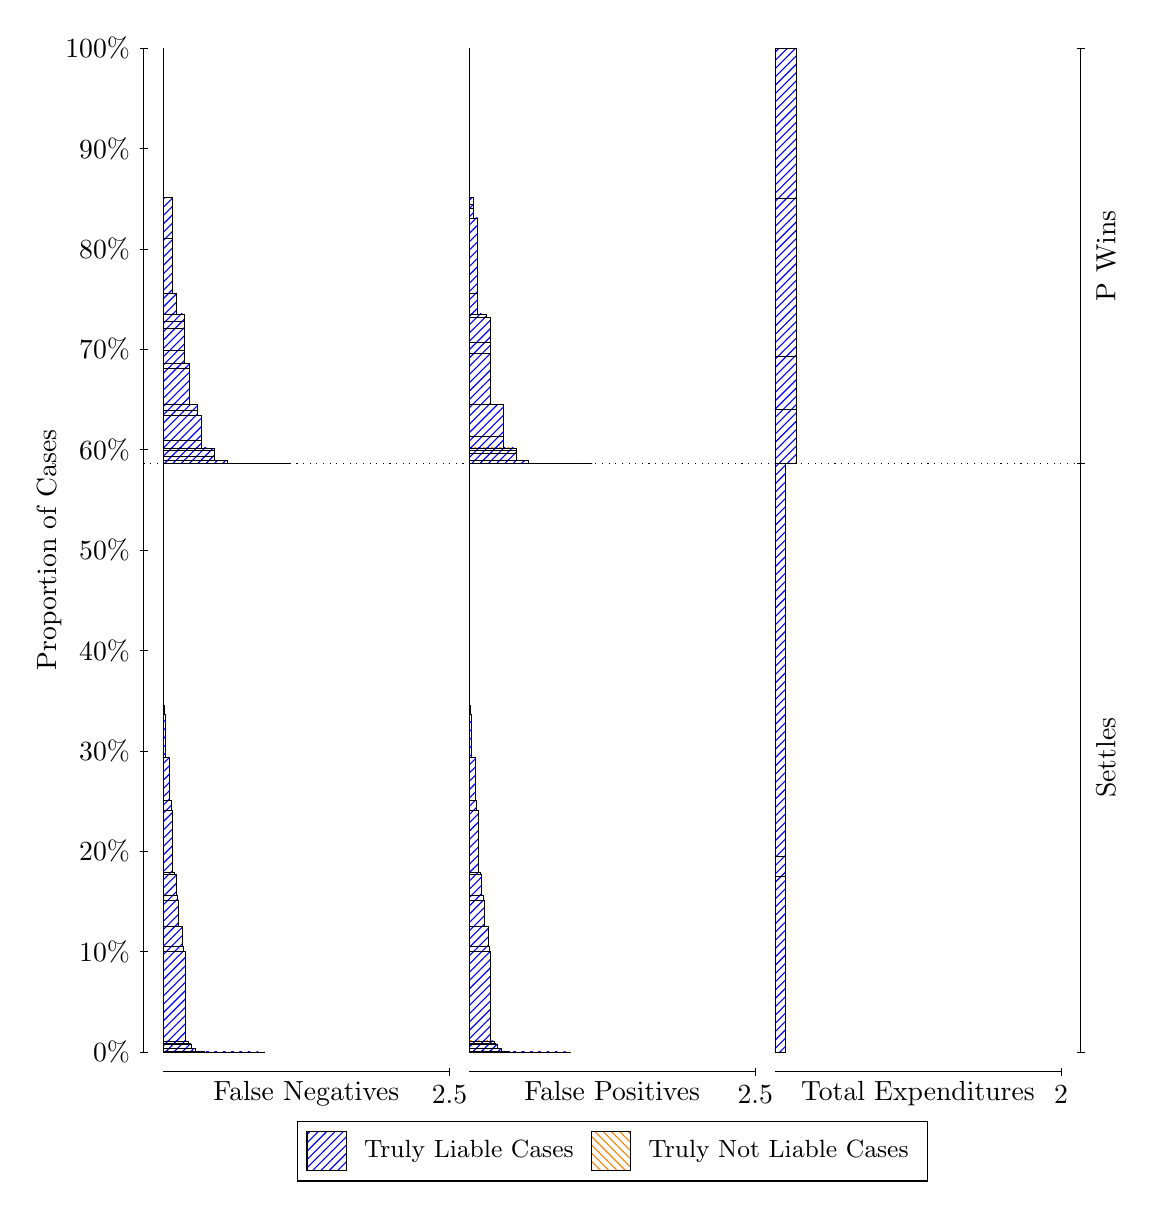
\begin{tikzpicture}
\draw[black, very thin] (1.5,1.75) -- (1.5,14.5);
\node[rotate=90, text=black, anchor=center] at (0.3, 8.125) {Proportion of Cases};
\draw[black, very thin] (1.45,1.75) -- (1.55,1.75);
\node[text=black, anchor=east] at (1.45, 1.75) {0\%};
\draw[black, very thin] (1.45,3.025) -- (1.55,3.025);
\node[text=black, anchor=east] at (1.45, 3.025) {10\%};
\draw[black, very thin] (1.45,4.3) -- (1.55,4.3);
\node[text=black, anchor=east] at (1.45, 4.3) {20\%};
\draw[black, very thin] (1.45,5.575) -- (1.55,5.575);
\node[text=black, anchor=east] at (1.45, 5.575) {30\%};
\draw[black, very thin] (1.45,6.85) -- (1.55,6.85);
\node[text=black, anchor=east] at (1.45, 6.85) {40\%};
\draw[black, very thin] (1.45,8.125) -- (1.55,8.125);
\node[text=black, anchor=east] at (1.45, 8.125) {50\%};
\draw[black, very thin] (1.45,9.4) -- (1.55,9.4);
\node[text=black, anchor=east] at (1.45, 9.4) {60\%};
\draw[black, very thin] (1.45,10.675) -- (1.55,10.675);
\node[text=black, anchor=east] at (1.45, 10.675) {70\%};
\draw[black, very thin] (1.45,11.95) -- (1.55,11.95);
\node[text=black, anchor=east] at (1.45, 11.95) {80\%};
\draw[black, very thin] (1.45,13.225) -- (1.55,13.225);
\node[text=black, anchor=east] at (1.45, 13.225) {90\%};
\draw[black, very thin] (1.45,14.5) -- (1.55,14.5);
\node[text=black, anchor=east] at (1.45, 14.5) {100\%};

\draw[black, very thin] (13.4,1.75) -- (13.4,14.5);
\draw[black, very thin] (13.35,1.75) -- (13.45,1.75);
\node[anchor=west] at (13.35, 1.75) {};
\draw[black, very thin] (13.35,9.224) -- (13.45,9.224);
\node[anchor=west] at (13.35, 9.224) {};
\draw[black, very thin] (13.35,14.5) -- (13.45,14.5);
\node[anchor=west] at (13.35, 14.5) {};

\draw[black, very thin, pattern color=blue, pattern=north east lines] (1.75,1.75) rectangle (3.0398,1.75);
\draw[black, very thin, pattern color=blue, pattern=north east lines] (1.75,1.75) rectangle (2.8945,1.75);
\draw[black, very thin, pattern color=blue, pattern=north east lines] (1.75,1.75) rectangle (2.8784,1.75);
\draw[black, very thin, pattern color=blue, pattern=north east lines] (1.75,1.75) rectangle (2.7492,1.75);
\draw[black, very thin, pattern color=blue, pattern=north east lines] (1.75,1.75) rectangle (2.733,1.75);
\draw[black, very thin, pattern color=blue, pattern=north east lines] (1.75,1.75) rectangle (2.7169,1.75);
\draw[black, very thin, pattern color=blue, pattern=north east lines] (1.75,1.75) rectangle (2.6765,1.75);
\draw[black, very thin, pattern color=blue, pattern=north east lines] (1.75,1.75) rectangle (2.5877,1.75);
\draw[black, very thin, pattern color=blue, pattern=north east lines] (1.75,1.75) rectangle (2.5715,1.75);
\draw[black, very thin, pattern color=blue, pattern=north east lines] (1.75,1.75) rectangle (2.5554,1.75);
\draw[black, very thin, pattern color=blue, pattern=north east lines] (1.75,1.75) rectangle (2.5312,1.75);
\draw[black, very thin, pattern color=blue, pattern=north east lines] (1.75,1.75) rectangle (2.515,1.75);
\draw[black, very thin, pattern color=blue, pattern=north east lines] (1.75,1.75) rectangle (2.4262,1.75);
\draw[black, very thin, pattern color=blue, pattern=north east lines] (1.75,1.75) rectangle (2.4101,1.75);
\draw[black, very thin, pattern color=blue, pattern=north east lines] (1.75,1.75) rectangle (2.3939,1.75);
\draw[black, very thin, pattern color=blue, pattern=north east lines] (1.75,1.75) rectangle (2.3858,1.75);
\draw[black, very thin, pattern color=blue, pattern=north east lines] (1.75,1.75) rectangle (2.3697,1.75);
\draw[black, very thin, pattern color=blue, pattern=north east lines] (1.75,1.75) rectangle (2.3535,1.75);
\draw[black, very thin, pattern color=blue, pattern=north east lines] (1.75,1.75) rectangle (2.3132,1.7511);
\draw[black, very thin, pattern color=blue, pattern=north east lines] (1.75,1.7511) rectangle (2.2647,1.7536);
\draw[black, very thin, pattern color=blue, pattern=north east lines] (1.75,1.7536) rectangle (2.2486,1.7538);
\draw[black, very thin, pattern color=blue, pattern=north east lines] (1.75,1.7538) rectangle (2.2324,1.7543);
\draw[black, very thin, pattern color=blue, pattern=north east lines] (1.75,1.7543) rectangle (2.2244,1.7543);
\draw[black, very thin, pattern color=blue, pattern=north east lines] (1.75,1.7543) rectangle (2.2082,1.7545);
\draw[black, very thin, pattern color=blue, pattern=north east lines] (1.75,1.7545) rectangle (2.1921,1.7545);
\draw[black, very thin, pattern color=blue, pattern=north east lines] (1.75,1.7545) rectangle (2.1678,1.7648);
\draw[black, very thin, pattern color=blue, pattern=north east lines] (1.75,1.7648) rectangle (2.1517,1.7944);
\draw[black, very thin, pattern color=blue, pattern=north east lines] (1.75,1.7944) rectangle (2.1032,1.8526);
\draw[black, very thin, pattern color=blue, pattern=north east lines] (1.75,1.8526) rectangle (2.0871,1.8594);
\draw[black, very thin, pattern color=blue, pattern=north east lines] (1.75,1.8594) rectangle (2.0709,1.8856);
\draw[black, very thin, pattern color=blue, pattern=north east lines] (1.75,1.8856) rectangle (2.0629,1.8857);
\draw[black, very thin, pattern color=blue, pattern=north east lines] (1.75,1.8857) rectangle (2.0467,1.8907);
\draw[black, very thin, pattern color=blue, pattern=north east lines] (1.75,1.8907) rectangle (2.0306,1.8907);
\draw[black, very thin, pattern color=blue, pattern=north east lines] (1.75,1.8907) rectangle (2.0225,3.0322);
\draw[black, very thin, pattern color=blue, pattern=north east lines] (1.75,3.0322) rectangle (2.0064,3.0933);
\draw[black, very thin, pattern color=blue, pattern=north east lines] (1.75,3.0933) rectangle (1.9902,3.342);
\draw[black, very thin, pattern color=blue, pattern=north east lines] (1.75,3.342) rectangle (1.9418,3.6759);
\draw[black, very thin, pattern color=blue, pattern=north east lines] (1.75,3.6759) rectangle (1.9256,3.7341);
\draw[black, very thin, pattern color=blue, pattern=north east lines] (1.75,3.7341) rectangle (1.9095,4.0016);
\draw[black, very thin, pattern color=blue, pattern=north east lines] (1.75,4.0016) rectangle (1.9014,4.0021);
\draw[black, very thin, pattern color=blue, pattern=north east lines] (1.75,4.0021) rectangle (1.8852,4.0278);
\draw[black, very thin, pattern color=blue, pattern=north east lines] (1.75,4.0278) rectangle (1.8691,4.0283);
\draw[black, very thin, pattern color=blue, pattern=north east lines] (1.75,4.0283) rectangle (1.861,4.8207);
\draw[black, very thin, pattern color=blue, pattern=north east lines] (1.75,4.8207) rectangle (1.8449,4.941);
\draw[black, very thin, pattern color=blue, pattern=north east lines] (1.75,4.941) rectangle (1.8287,5.487);
\draw[black, very thin, pattern color=blue, pattern=north east lines] (1.75,5.487) rectangle (1.7803,6.033);
\draw[black, very thin, pattern color=blue, pattern=north east lines] (1.75,6.033) rectangle (1.7641,6.1534);
\draw[black, very thin, pattern color=orange, pattern=north west lines] (1.75,6.1534) rectangle (1.75,6.1534);
\draw[black, very thin, pattern color=blue, pattern=north east lines] (1.75,6.1534) rectangle (1.75,9.224);
\draw[black, very thin, pattern color=blue, pattern=north east lines] (1.75,9.224) rectangle (3.3668,9.224);
\draw[black, very thin, pattern color=blue, pattern=north east lines] (1.75,9.224) rectangle (3.2054,9.224);
\draw[black, very thin, pattern color=blue, pattern=north east lines] (1.75,9.224) rectangle (3.0439,9.224);
\draw[black, very thin, pattern color=blue, pattern=north east lines] (1.75,9.224) rectangle (2.9894,9.224);
\draw[black, very thin, pattern color=blue, pattern=north east lines] (1.75,9.224) rectangle (2.8824,9.2241);
\draw[black, very thin, pattern color=blue, pattern=north east lines] (1.75,9.2241) rectangle (2.8824,9.2242);
\draw[black, very thin, pattern color=blue, pattern=north east lines] (1.75,9.2242) rectangle (2.8279,9.2242);
\draw[black, very thin, pattern color=blue, pattern=north east lines] (1.75,9.2242) rectangle (2.7209,9.2263);
\draw[black, very thin, pattern color=blue, pattern=north east lines] (1.75,9.2263) rectangle (2.7209,9.2277);
\draw[black, very thin, pattern color=blue, pattern=north east lines] (1.75,9.2277) rectangle (2.6664,9.2277);
\draw[black, very thin, pattern color=blue, pattern=north east lines] (1.75,9.2277) rectangle (2.5594,9.2587);
\draw[black, very thin, pattern color=blue, pattern=north east lines] (1.75,9.2587) rectangle (2.5049,9.2587);
\draw[black, very thin, pattern color=blue, pattern=north east lines] (1.75,9.2587) rectangle (2.5049,9.2588);
\draw[black, very thin, pattern color=blue, pattern=north east lines] (1.75,9.2588) rectangle (2.3979,9.3128);
\draw[black, very thin, pattern color=blue, pattern=north east lines] (1.75,9.3128) rectangle (2.3979,9.3939);
\draw[black, very thin, pattern color=blue, pattern=north east lines] (1.75,9.3939) rectangle (2.3979,9.4112);
\draw[black, very thin, pattern color=blue, pattern=north east lines] (1.75,9.4112) rectangle (2.3434,9.4149);
\draw[black, very thin, pattern color=blue, pattern=north east lines] (1.75,9.4149) rectangle (2.3434,9.4223);
\draw[black, very thin, pattern color=blue, pattern=north east lines] (1.75,9.4223) rectangle (2.3434,9.4227);
\draw[black, very thin, pattern color=blue, pattern=north east lines] (1.75,9.4227) rectangle (2.2365,9.5161);
\draw[black, very thin, pattern color=blue, pattern=north east lines] (1.75,9.5161) rectangle (2.2365,9.8384);
\draw[black, very thin, pattern color=blue, pattern=north east lines] (1.75,9.8384) rectangle (2.182,9.8392);
\draw[black, very thin, pattern color=blue, pattern=north east lines] (1.75,9.8392) rectangle (2.182,9.9024);
\draw[black, very thin, pattern color=blue, pattern=north east lines] (1.75,9.9024) rectangle (2.182,9.9755);
\draw[black, very thin, pattern color=blue, pattern=north east lines] (1.75,9.9755) rectangle (2.075,9.9809);
\draw[black, very thin, pattern color=blue, pattern=north east lines] (1.75,9.9809) rectangle (2.075,10.439);
\draw[black, very thin, pattern color=blue, pattern=north east lines] (1.75,10.439) rectangle (2.075,10.492);
\draw[black, very thin, pattern color=blue, pattern=north east lines] (1.75,10.492) rectangle (2.0205,10.665);
\draw[black, very thin, pattern color=blue, pattern=north east lines] (1.75,10.665) rectangle (2.0205,10.943);
\draw[black, very thin, pattern color=blue, pattern=north east lines] (1.75,10.943) rectangle (2.0205,11.027);
\draw[black, very thin, pattern color=blue, pattern=north east lines] (1.75,11.027) rectangle (2.0205,11.125);
\draw[black, very thin, pattern color=blue, pattern=north east lines] (1.75,11.125) rectangle (1.9135,11.382);
\draw[black, very thin, pattern color=blue, pattern=north east lines] (1.75,11.382) rectangle (1.859,12.084);
\draw[black, very thin, pattern color=blue, pattern=north east lines] (1.75,12.084) rectangle (1.859,12.599);
\draw[black, very thin, pattern color=blue, pattern=north east lines] (1.75,12.599) rectangle (1.752,12.646);
\draw[black, very thin, pattern color=blue, pattern=north east lines] (1.75,12.646) rectangle (1.752,12.646);
\draw[black, very thin, pattern color=orange, pattern=north west lines] (1.75,12.646) rectangle (1.75,12.646);
\draw[black, very thin, pattern color=blue, pattern=north east lines] (1.75,12.646) rectangle (1.75,14.5);
\draw[black, very thin, pattern color=orange, pattern=north west lines] (5.6333,1.75) rectangle (6.9232,1.75);
\draw[black, very thin, pattern color=blue, pattern=north east lines] (5.6333,1.75) rectangle (6.9232,1.75);
\draw[black, very thin, pattern color=orange, pattern=north west lines] (5.6333,1.75) rectangle (6.7778,1.75);
\draw[black, very thin, pattern color=blue, pattern=north east lines] (5.6333,1.75) rectangle (6.7778,1.75);
\draw[black, very thin, pattern color=blue, pattern=north east lines] (5.6333,1.75) rectangle (6.7617,1.75);
\draw[black, very thin, pattern color=orange, pattern=north west lines] (5.6333,1.75) rectangle (6.6325,1.75);
\draw[black, very thin, pattern color=blue, pattern=north east lines] (5.6333,1.75) rectangle (6.6325,1.75);
\draw[black, very thin, pattern color=blue, pattern=north east lines] (5.6333,1.75) rectangle (6.6164,1.75);
\draw[black, very thin, pattern color=blue, pattern=north east lines] (5.6333,1.75) rectangle (6.6002,1.75);
\draw[black, very thin, pattern color=orange, pattern=north west lines] (5.6333,1.75) rectangle (6.5598,1.75);
\draw[black, very thin, pattern color=blue, pattern=north east lines] (5.6333,1.75) rectangle (6.5598,1.75);
\draw[black, very thin, pattern color=blue, pattern=north east lines] (5.6333,1.75) rectangle (6.471,1.75);
\draw[black, very thin, pattern color=blue, pattern=north east lines] (5.6333,1.75) rectangle (6.4549,1.75);
\draw[black, very thin, pattern color=blue, pattern=north east lines] (5.6333,1.75) rectangle (6.4387,1.75);
\draw[black, very thin, pattern color=orange, pattern=north west lines] (5.6333,1.75) rectangle (6.4145,1.75);
\draw[black, very thin, pattern color=blue, pattern=north east lines] (5.6333,1.75) rectangle (6.4145,1.75);
\draw[black, very thin, pattern color=blue, pattern=north east lines] (5.6333,1.75) rectangle (6.3984,1.75);
\draw[black, very thin, pattern color=blue, pattern=north east lines] (5.6333,1.75) rectangle (6.3095,1.75);
\draw[black, very thin, pattern color=blue, pattern=north east lines] (5.6333,1.75) rectangle (6.2934,1.75);
\draw[black, very thin, pattern color=blue, pattern=north east lines] (5.6333,1.75) rectangle (6.2772,1.75);
\draw[black, very thin, pattern color=orange, pattern=north west lines] (5.6333,1.75) rectangle (6.2692,1.75);
\draw[black, very thin, pattern color=blue, pattern=north east lines] (5.6333,1.75) rectangle (6.2692,1.75);
\draw[black, very thin, pattern color=blue, pattern=north east lines] (5.6333,1.75) rectangle (6.253,1.75);
\draw[black, very thin, pattern color=blue, pattern=north east lines] (5.6333,1.75) rectangle (6.2369,1.75);
\draw[black, very thin, pattern color=orange, pattern=north west lines] (5.6333,1.75) rectangle (6.1965,1.75);
\draw[black, very thin, pattern color=blue, pattern=north east lines] (5.6333,1.75) rectangle (6.1965,1.7511);
\draw[black, very thin, pattern color=blue, pattern=north east lines] (5.6333,1.7511) rectangle (6.1481,1.7536);
\draw[black, very thin, pattern color=blue, pattern=north east lines] (5.6333,1.7536) rectangle (6.1319,1.7538);
\draw[black, very thin, pattern color=blue, pattern=north east lines] (5.6333,1.7538) rectangle (6.1158,1.7543);
\draw[black, very thin, pattern color=blue, pattern=north east lines] (5.6333,1.7543) rectangle (6.1077,1.7543);
\draw[black, very thin, pattern color=blue, pattern=north east lines] (5.6333,1.7543) rectangle (6.0915,1.7545);
\draw[black, very thin, pattern color=blue, pattern=north east lines] (5.6333,1.7545) rectangle (6.0754,1.7545);
\draw[black, very thin, pattern color=orange, pattern=north west lines] (5.6333,1.7545) rectangle (6.0512,1.7545);
\draw[black, very thin, pattern color=blue, pattern=north east lines] (5.6333,1.7545) rectangle (6.0512,1.7648);
\draw[black, very thin, pattern color=blue, pattern=north east lines] (5.6333,1.7648) rectangle (6.035,1.7944);
\draw[black, very thin, pattern color=blue, pattern=north east lines] (5.6333,1.7944) rectangle (5.9866,1.8526);
\draw[black, very thin, pattern color=blue, pattern=north east lines] (5.6333,1.8526) rectangle (5.9704,1.8594);
\draw[black, very thin, pattern color=blue, pattern=north east lines] (5.6333,1.8594) rectangle (5.9543,1.8856);
\draw[black, very thin, pattern color=blue, pattern=north east lines] (5.6333,1.8856) rectangle (5.9462,1.8857);
\draw[black, very thin, pattern color=blue, pattern=north east lines] (5.6333,1.8857) rectangle (5.9301,1.8906);
\draw[black, very thin, pattern color=blue, pattern=north east lines] (5.6333,1.8906) rectangle (5.9139,1.8907);
\draw[black, very thin, pattern color=orange, pattern=north west lines] (5.6333,1.8907) rectangle (5.9058,1.8907);
\draw[black, very thin, pattern color=blue, pattern=north east lines] (5.6333,1.8907) rectangle (5.9058,3.0322);
\draw[black, very thin, pattern color=blue, pattern=north east lines] (5.6333,3.0322) rectangle (5.8897,3.0933);
\draw[black, very thin, pattern color=blue, pattern=north east lines] (5.6333,3.0933) rectangle (5.8735,3.3419);
\draw[black, very thin, pattern color=blue, pattern=north east lines] (5.6333,3.3419) rectangle (5.8251,3.6759);
\draw[black, very thin, pattern color=blue, pattern=north east lines] (5.6333,3.6759) rectangle (5.8089,3.7341);
\draw[black, very thin, pattern color=blue, pattern=north east lines] (5.6333,3.7341) rectangle (5.7928,4.0015);
\draw[black, very thin, pattern color=blue, pattern=north east lines] (5.6333,4.0015) rectangle (5.7847,4.002);
\draw[black, very thin, pattern color=blue, pattern=north east lines] (5.6333,4.002) rectangle (5.7686,4.0277);
\draw[black, very thin, pattern color=blue, pattern=north east lines] (5.6333,4.0277) rectangle (5.7524,4.0282);
\draw[black, very thin, pattern color=blue, pattern=north east lines] (5.6333,4.0282) rectangle (5.7444,4.8206);
\draw[black, very thin, pattern color=blue, pattern=north east lines] (5.6333,4.8206) rectangle (5.7282,4.9409);
\draw[black, very thin, pattern color=blue, pattern=north east lines] (5.6333,4.9409) rectangle (5.7121,5.487);
\draw[black, very thin, pattern color=blue, pattern=north east lines] (5.6333,5.487) rectangle (5.6636,6.033);
\draw[black, very thin, pattern color=blue, pattern=north east lines] (5.6333,6.033) rectangle (5.6475,6.1533);
\draw[black, very thin, pattern color=blue, pattern=north east lines] (5.6333,6.1533) rectangle (5.6333,9.224);
\draw[black, very thin, pattern color=orange, pattern=north west lines] (5.6333,9.224) rectangle (7.1957,9.224);
\draw[black, very thin, pattern color=blue, pattern=north east lines] (5.6333,9.224) rectangle (7.1957,9.224);
\draw[black, very thin, pattern color=orange, pattern=north west lines] (5.6333,9.224) rectangle (7.0342,9.224);
\draw[black, very thin, pattern color=blue, pattern=north east lines] (5.6333,9.224) rectangle (7.0342,9.224);
\draw[black, very thin, pattern color=orange, pattern=north west lines] (5.6333,9.224) rectangle (6.8727,9.224);
\draw[black, very thin, pattern color=blue, pattern=north east lines] (5.6333,9.224) rectangle (6.8727,9.224);
\draw[black, very thin, pattern color=blue, pattern=north east lines] (5.6333,9.224) rectangle (6.8727,9.224);
\draw[black, very thin, pattern color=blue, pattern=north east lines] (5.6333,9.224) rectangle (6.7112,9.2241);
\draw[black, very thin, pattern color=orange, pattern=north west lines] (5.6333,9.2241) rectangle (6.7112,9.2241);
\draw[black, very thin, pattern color=blue, pattern=north east lines] (5.6333,9.2241) rectangle (6.7112,9.2242);
\draw[black, very thin, pattern color=orange, pattern=north west lines] (5.6333,9.2242) rectangle (6.5497,9.2242);
\draw[black, very thin, pattern color=blue, pattern=north east lines] (5.6333,9.2242) rectangle (6.5497,9.2277);
\draw[black, very thin, pattern color=orange, pattern=north west lines] (5.6333,9.2277) rectangle (6.4952,9.2277);
\draw[black, very thin, pattern color=blue, pattern=north east lines] (5.6333,9.2277) rectangle (6.4952,9.2277);
\draw[black, very thin, pattern color=orange, pattern=north west lines] (5.6333,9.2277) rectangle (6.3883,9.2277);
\draw[black, very thin, pattern color=blue, pattern=north east lines] (5.6333,9.2277) rectangle (6.3883,9.2588);
\draw[black, very thin, pattern color=blue, pattern=north east lines] (5.6333,9.2588) rectangle (6.3338,9.2588);
\draw[black, very thin, pattern color=orange, pattern=north west lines] (5.6333,9.2588) rectangle (6.3338,9.2588);
\draw[black, very thin, pattern color=blue, pattern=north east lines] (5.6333,9.2588) rectangle (6.3338,9.2588);
\draw[black, very thin, pattern color=orange, pattern=north west lines] (5.6333,9.2588) rectangle (6.2268,9.2588);
\draw[black, very thin, pattern color=blue, pattern=north east lines] (5.6333,9.2588) rectangle (6.2268,9.3483);
\draw[black, very thin, pattern color=blue, pattern=north east lines] (5.6333,9.3483) rectangle (6.2268,9.3904);
\draw[black, very thin, pattern color=blue, pattern=north east lines] (5.6333,9.3904) rectangle (6.2268,9.4227);
\draw[black, very thin, pattern color=blue, pattern=north east lines] (5.6333,9.4227) rectangle (6.1723,9.4227);
\draw[black, very thin, pattern color=orange, pattern=north west lines] (5.6333,9.4227) rectangle (6.1723,9.4227);
\draw[black, very thin, pattern color=blue, pattern=north east lines] (5.6333,9.4227) rectangle (6.1723,9.4227);
\draw[black, very thin, pattern color=orange, pattern=north west lines] (5.6333,9.4227) rectangle (6.0653,9.4227);
\draw[black, very thin, pattern color=blue, pattern=north east lines] (5.6333,9.4227) rectangle (6.0653,9.567);
\draw[black, very thin, pattern color=blue, pattern=north east lines] (5.6333,9.567) rectangle (6.0653,9.9754);
\draw[black, very thin, pattern color=blue, pattern=north east lines] (5.6333,9.9754) rectangle (6.0108,9.9754);
\draw[black, very thin, pattern color=orange, pattern=north west lines] (5.6333,9.9754) rectangle (6.0108,9.9754);
\draw[black, very thin, pattern color=blue, pattern=north east lines] (5.6333,9.9754) rectangle (6.0108,9.9755);
\draw[black, very thin, pattern color=blue, pattern=north east lines] (5.6333,9.9755) rectangle (5.9038,10.622);
\draw[black, very thin, pattern color=blue, pattern=north east lines] (5.6333,10.622) rectangle (5.9038,10.757);
\draw[black, very thin, pattern color=blue, pattern=north east lines] (5.6333,10.757) rectangle (5.9038,11.078);
\draw[black, very thin, pattern color=blue, pattern=north east lines] (5.6333,11.078) rectangle (5.8493,11.078);
\draw[black, very thin, pattern color=orange, pattern=north west lines] (5.6333,11.078) rectangle (5.8493,11.078);
\draw[black, very thin, pattern color=blue, pattern=north east lines] (5.6333,11.078) rectangle (5.8493,11.119);
\draw[black, very thin, pattern color=blue, pattern=north east lines] (5.6333,11.119) rectangle (5.8493,11.125);
\draw[black, very thin, pattern color=blue, pattern=north east lines] (5.6333,11.125) rectangle (5.7423,11.389);
\draw[black, very thin, pattern color=blue, pattern=north east lines] (5.6333,11.389) rectangle (5.7423,12.342);
\draw[black, very thin, pattern color=blue, pattern=north east lines] (5.6333,12.342) rectangle (5.6878,12.463);
\draw[black, very thin, pattern color=orange, pattern=north west lines] (5.6333,12.463) rectangle (5.6878,12.463);
\draw[black, very thin, pattern color=blue, pattern=north east lines] (5.6333,12.463) rectangle (5.6878,12.514);
\draw[black, very thin, pattern color=blue, pattern=north east lines] (5.6333,12.514) rectangle (5.6878,12.599);
\draw[black, very thin, pattern color=blue, pattern=north east lines] (5.6333,12.599) rectangle (5.6333,14.5);
\draw[black, very thin, pattern color=orange, pattern=north west lines] (9.5167,1.75) rectangle (9.6529,1.75);
\draw[black, very thin, pattern color=blue, pattern=north east lines] (9.5167,1.75) rectangle (9.6529,3.978);
\draw[black, very thin, pattern color=orange, pattern=north west lines] (9.5167,3.978) rectangle (9.6529,3.978);
\draw[black, very thin, pattern color=blue, pattern=north east lines] (9.5167,3.978) rectangle (9.6529,4.235);
\draw[black, very thin, pattern color=orange, pattern=north west lines] (9.5167,4.235) rectangle (9.6529,4.235);
\draw[black, very thin, pattern color=blue, pattern=north east lines] (9.5167,4.235) rectangle (9.6529,9.224);
\draw[black, very thin, pattern color=orange, pattern=north west lines] (9.5167,9.224) rectangle (9.7892,9.224);
\draw[black, very thin, pattern color=blue, pattern=north east lines] (9.5167,9.224) rectangle (9.7892,9.9089);
\draw[black, very thin, pattern color=orange, pattern=north west lines] (9.5167,9.9089) rectangle (9.7892,9.9089);
\draw[black, very thin, pattern color=blue, pattern=north east lines] (9.5167,9.9089) rectangle (9.7892,10.58);
\draw[black, very thin, pattern color=orange, pattern=north west lines] (9.5167,10.58) rectangle (9.7892,10.58);
\draw[black, very thin, pattern color=blue, pattern=north east lines] (9.5167,10.58) rectangle (9.7892,12.593);
\draw[black, very thin, pattern color=orange, pattern=north west lines] (9.5167,12.593) rectangle (9.7892,12.593);
\draw[black, very thin, pattern color=blue, pattern=north east lines] (9.5167,12.593) rectangle (9.7892,14.5);
\draw[black, dotted] (1.5,9.224) -- (13.4,9.224);
\draw[black, very thin] (1.75,1.5) -- (5.3833,1.5);
\node[text=black, anchor=north] at (3.5667, 1.5) {False Negatives};
\draw[black, very thin] (5.3833,1.45) -- (5.3833,1.55);
\node[text=black, anchor=north] at (5.3833, 1.45) {2.5};

\draw[black, very thin] (5.6333,1.5) -- (9.2667,1.5);
\node[text=black, anchor=north] at (7.45, 1.5) {False Positives};
\draw[black, very thin] (9.2667,1.45) -- (9.2667,1.55);
\node[text=black, anchor=north] at (9.2667, 1.45) {2.5};

\draw[black, very thin] (9.5167,1.5) -- (13.15,1.5);
\node[text=black, anchor=north] at (11.333, 1.5) {Total Expenditures};
\draw[black, very thin] (13.15,1.45) -- (13.15,1.55);
\node[text=black, anchor=north] at (13.15, 1.45) {2};

\node[text=black, centered, rotate=90] at (13.72, 5.487) {Settles};
\node[text=black, centered, rotate=90] at (13.72, 11.862) {P Wins};

\draw (7.449999999999999,1.5) node[draw=none] (baseCoordinate) {};
\begin{scope}[align=center]
        \matrix[scale=0.5, draw=black, below=0.5cm of baseCoordinate, nodes={draw}, column sep=0.1cm]{
            \node[rectangle, draw, minimum width=0.5cm, minimum height=0.5cm, pattern color=blue, pattern=north east lines] {}; &
            \node[draw=none, font=\small, text=black] (B) {Truly Liable Cases}; &
            \node[rectangle, draw, minimum width=0.5cm, minimum height=0.5cm, pattern color=orange, pattern=north west lines] {}; &
            \node[draw=none, font=\small, text=black] (B) {Truly Not Liable Cases}; \\
            };
\end{scope}

\end{tikzpicture}
\end{document}